

\section{Urheberschaftsbestätigung}

Hiermit erkläre ich, dass die vorliegende Arbeit von mir eigenständig verfasst wurde und keine anderen als die von mir angegebenen Hilfsmittel verwendet wurden. Alle Stellen der Arbeit, die anderen Werken dem Wortlaut oder dem Sinn nach entnommen wurden, sind mit Angaben der Quellen als solche gekennzeichnet.

Ich nehme zur Kenntnis, dass Arbeiten, die unter Beizug unerlaubter Hilfsmittel verfasst wurden und die fremde Textteile ohne entsprechenden Herkunftsnachweis enthalten, verfolgt und geahndet werden.
\\
\\Zürich den 05. Februar 2015


\includegraphics[width=0.2\linewidth]{./graphics/UnterschriftDavid.pdf}\\
David Sichau



\section{Daten und Auswertungen}

Für die Auswertungen wurde offene Programmiersprache R\footnote{\url{http://www.r-project.org/}} verwendet. Diese ist für alle  Systeme kostenfrei verfügbar. Aller Code und die Daten dieser Masterarbeit befinden sich auf GitHub und sind frei verfügbar.
\github{http://git.io/buGR}



\section{Fragebogen}
Hier folgen die Fragebögen, welche die Schülerinnen und Schüler ausgefüllt haben. Da sie sich leicht unterschieden, wurden beide Fragebögen angehängt.

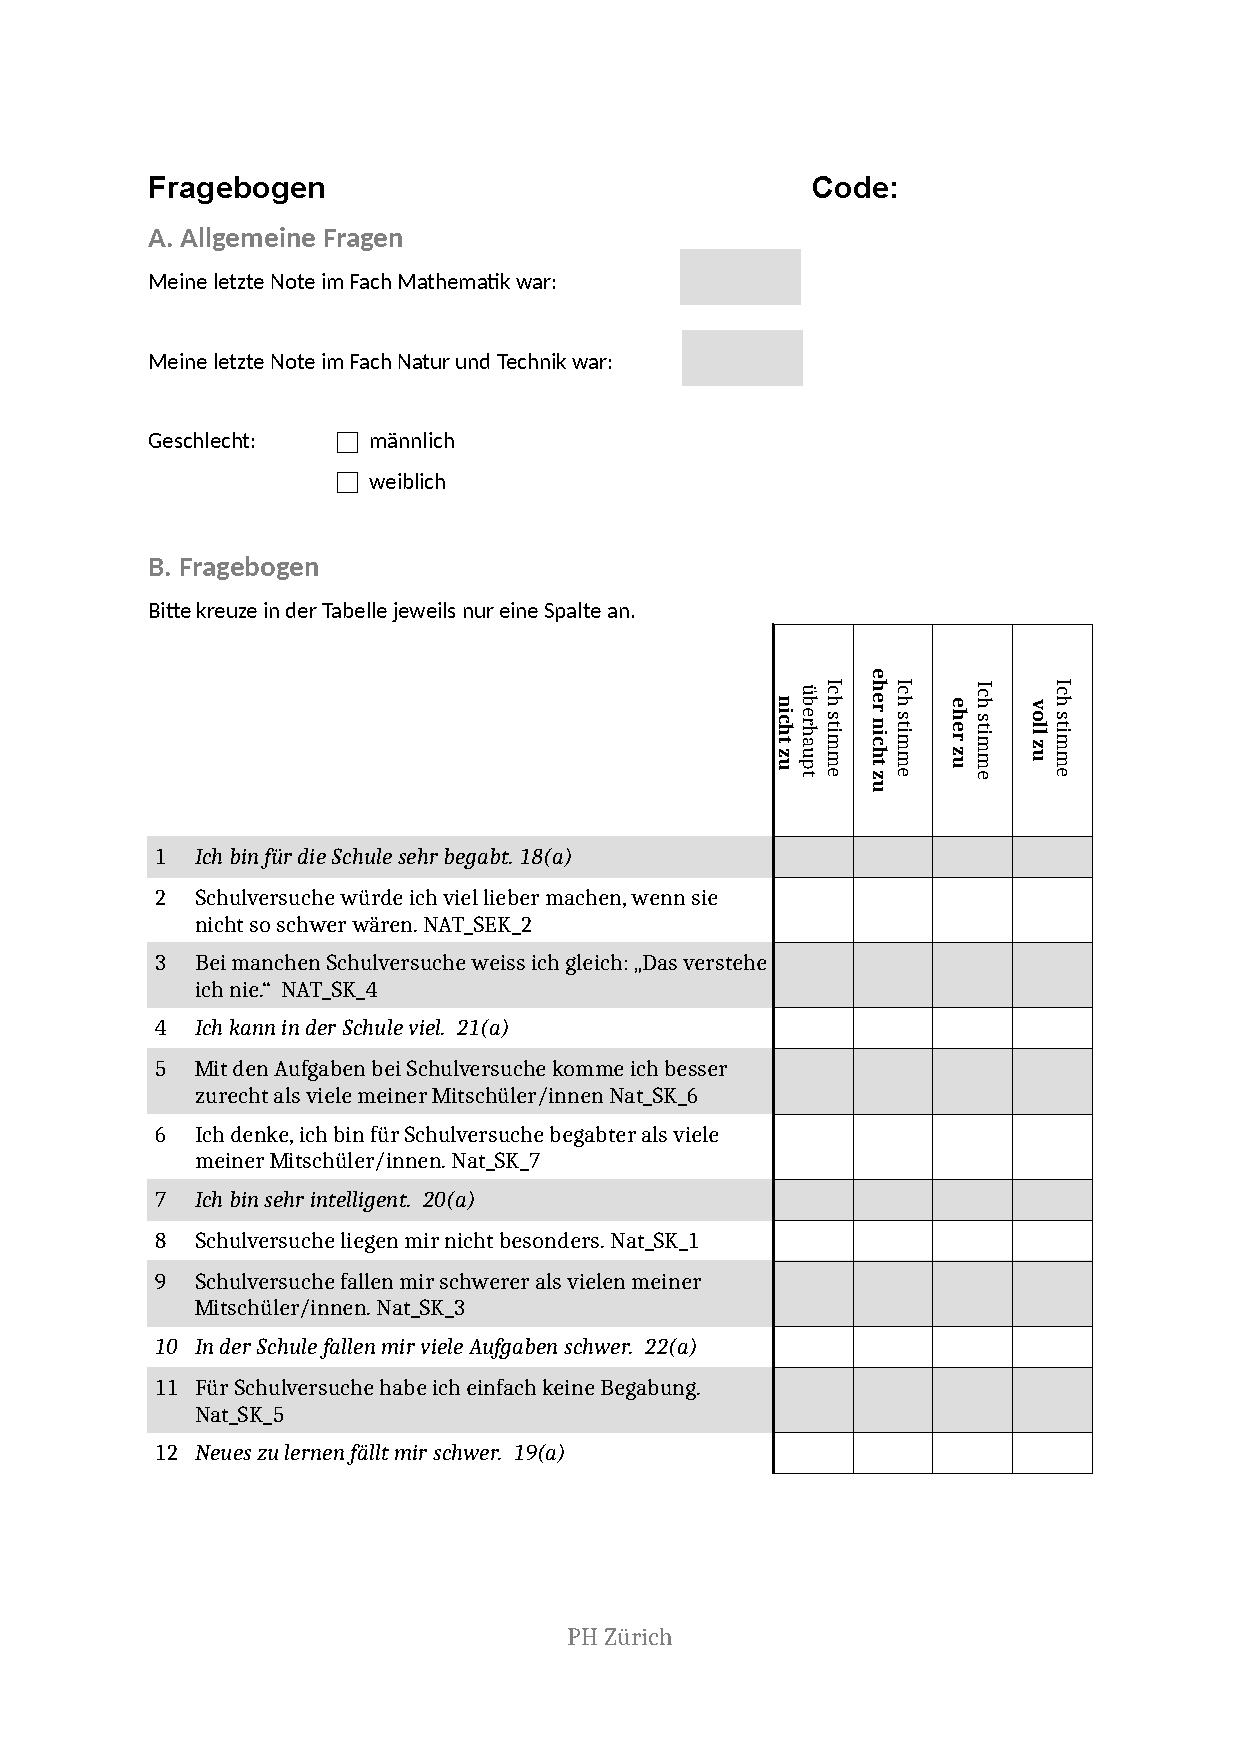
\includepdf[pages=1,pagecommand={\pagestyle{fancy}\subsection{Fragebogen am Anfang}},scale=0.8]{./graphics/Fragebogen_Anfang.pdf} 
\includepdf[pages=2-,pagecommand={\pagestyle{fancy}},scale=0.8]{./graphics/Fragebogen_Anfang.pdf} 
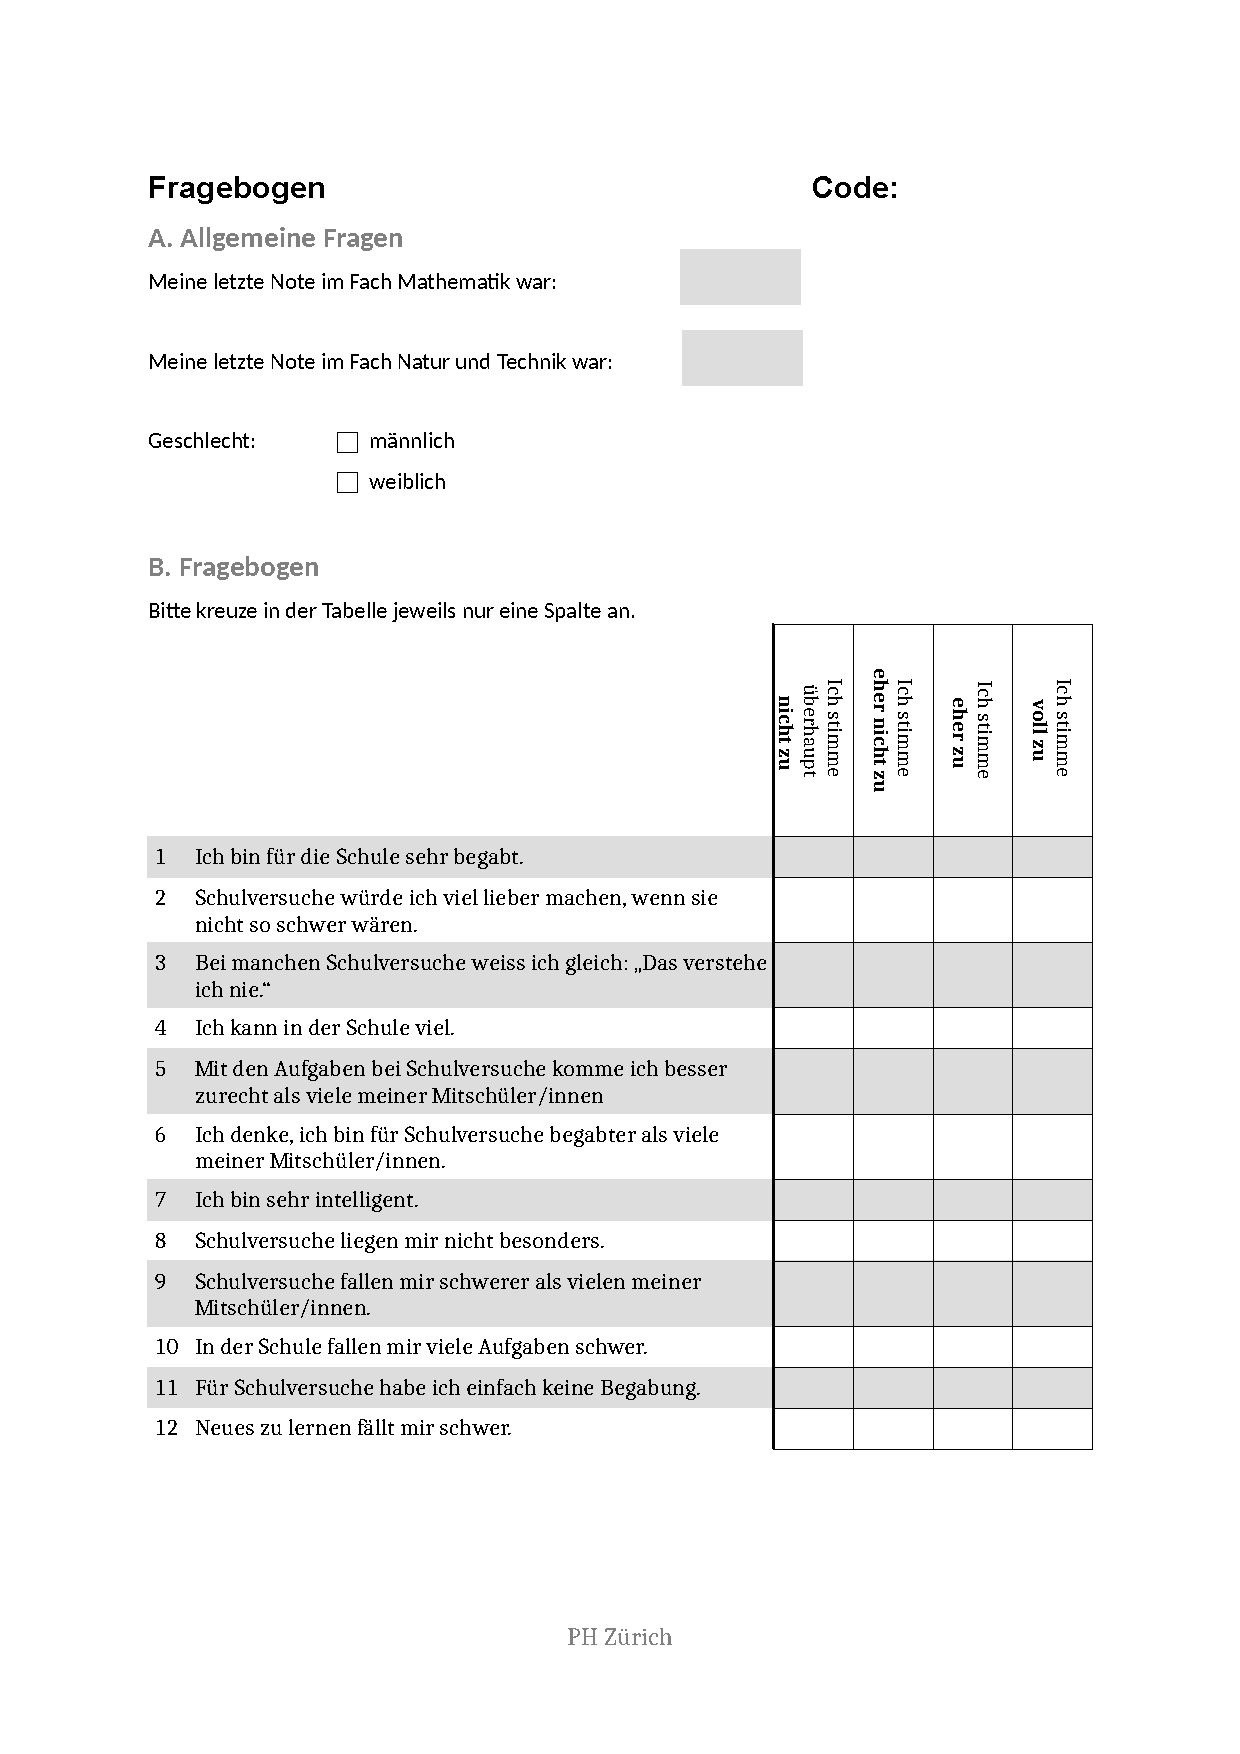
\includepdf[pages=1,pagecommand={\pagestyle{fancy}\subsection{Fragebogen am Ende}},scale=0.8]{./graphics/Fragebogen_Ende.pdf} 
\includepdf[pages=2-,pagecommand={\pagestyle{fancy}},scale=0.8]{./graphics/Fragebogen_Ende.pdf} 



\section{Aufgabenstellung und Kodierungen}
\label{sec:Kodierung}
Im folgenden Abschnitt befinden sich die Aufgabenstellungen der drei Tests und die Kodiermanuals.

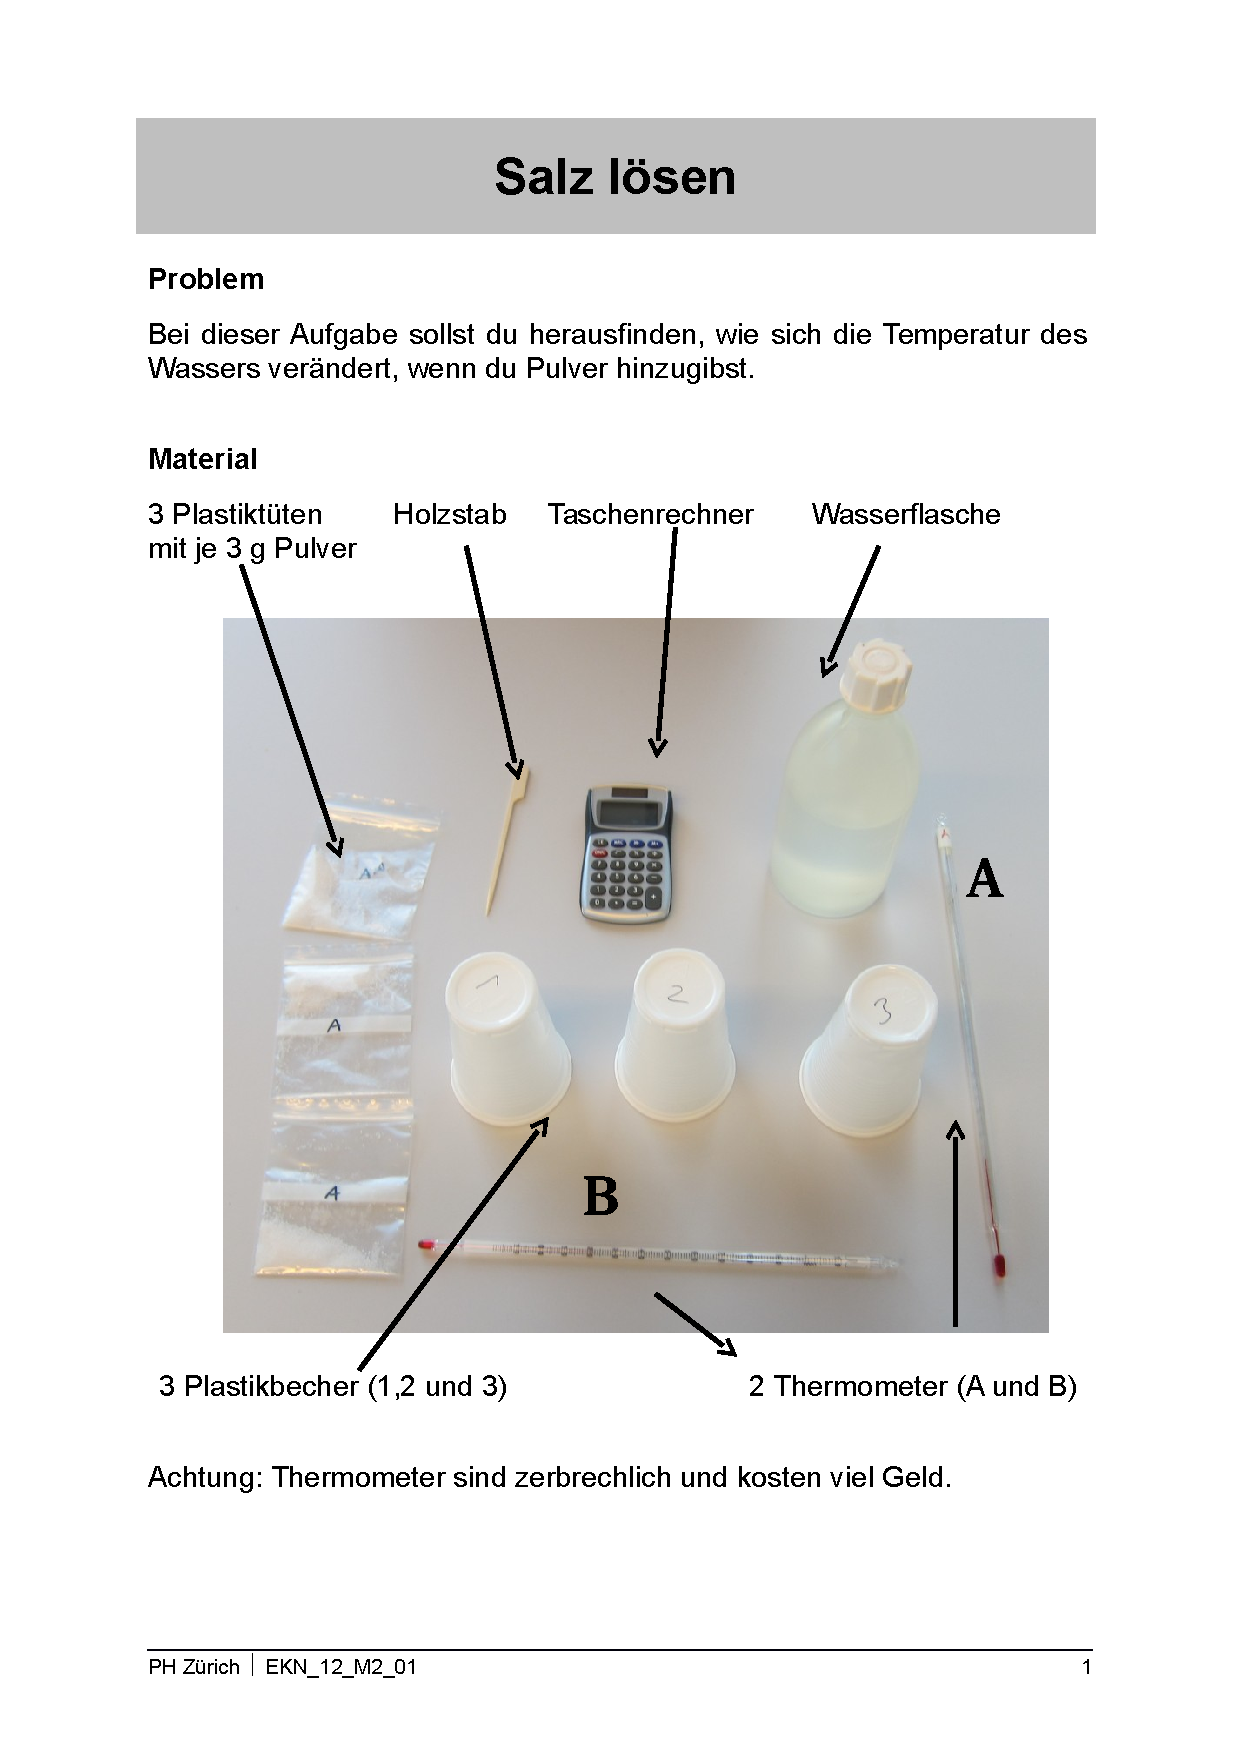
\includepdf[pages=1,pagecommand={
\pagestyle{fancy}
\subsection{Test 201: Aufgabenstellung}
},scale=0.8]{./graphics/Test_C.pdf} 
\includepdf[pages=2-,pagecommand={\pagestyle{fancy}},scale=0.8]{./graphics/Test_C.pdf} 

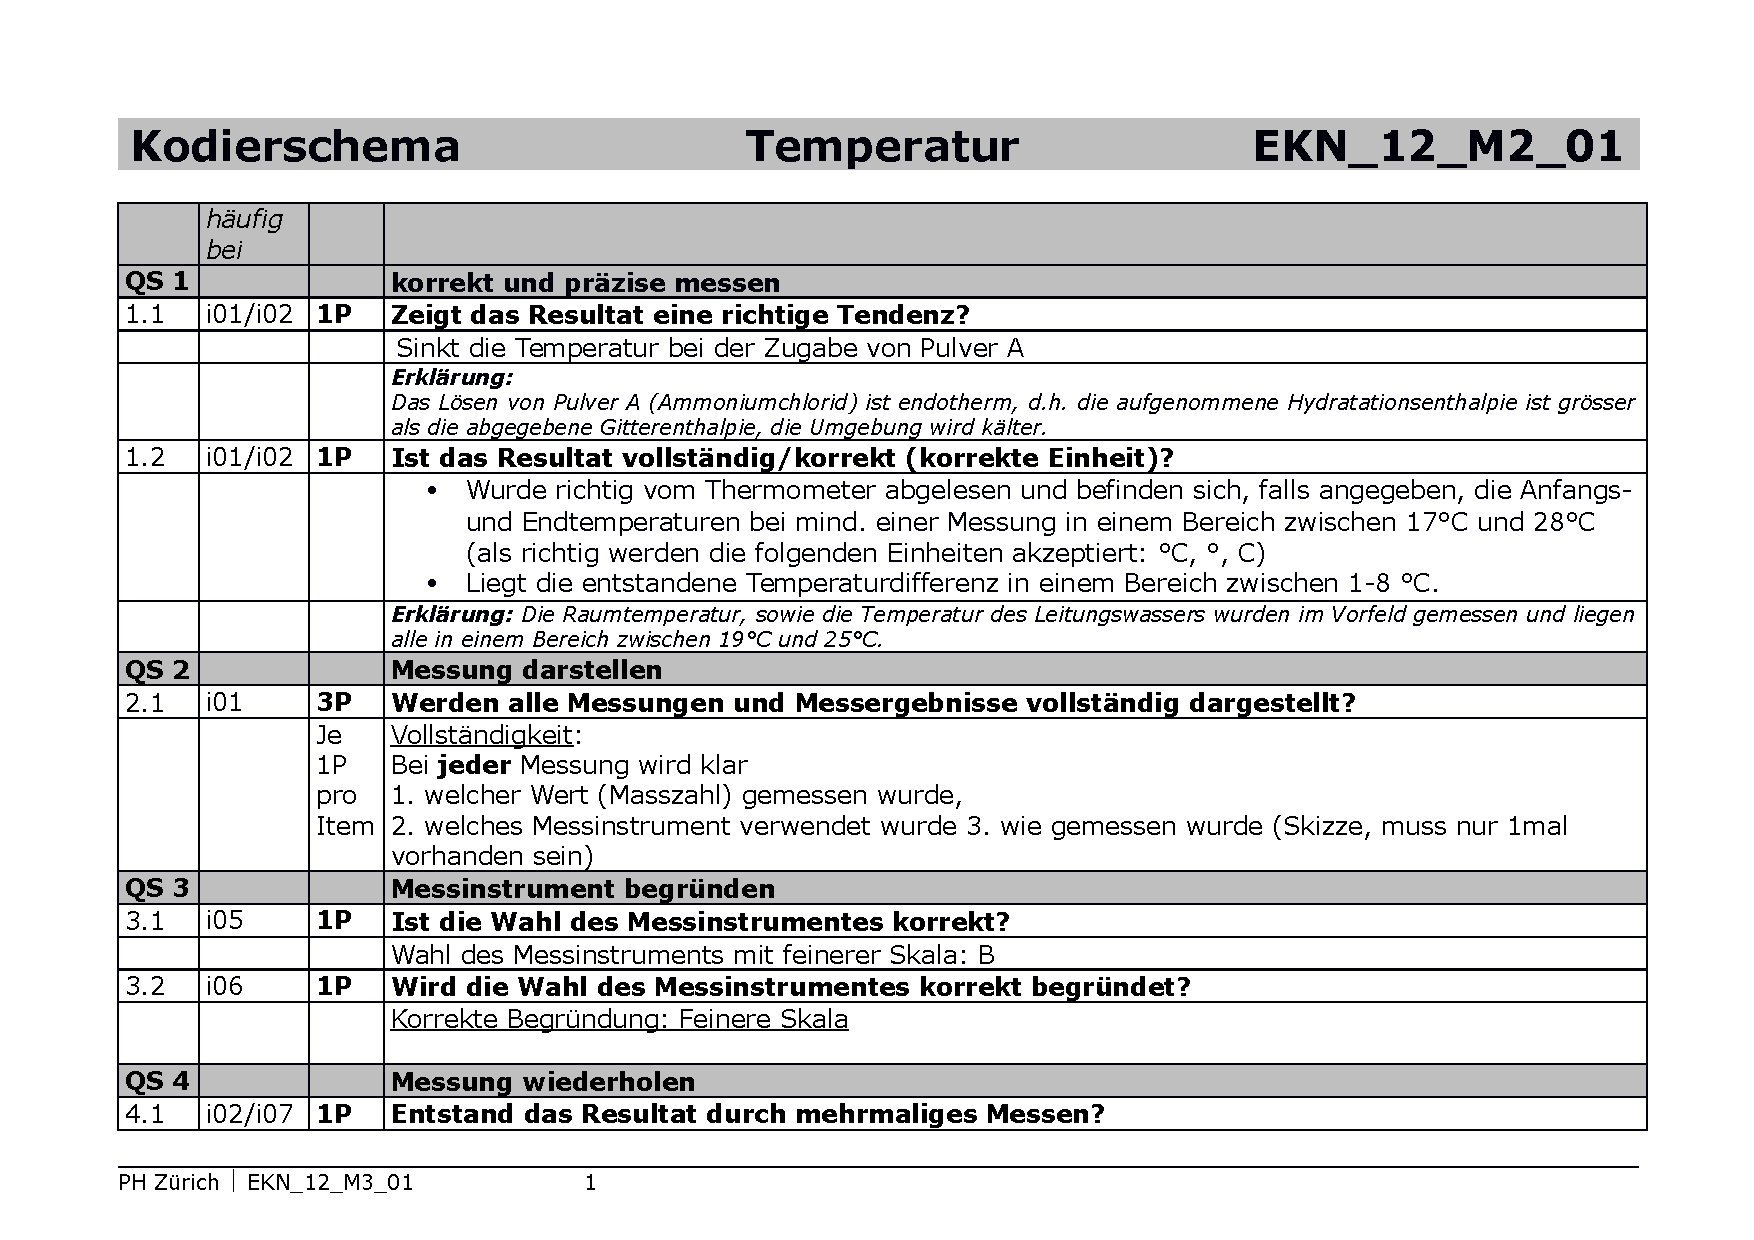
\includepdf[pages=1,pagecommand={\pagestyle{fancy}\subsection{Test 201: Kodierung}},scale=0.8]{./graphics/EKN_12_M2_Kodierschema_neu.pdf} 
\includepdf[pages=2-,pagecommand={\pagestyle{fancy}},scale=0.8]{./graphics/EKN_12_M2_Kodierschema_neu.pdf} 


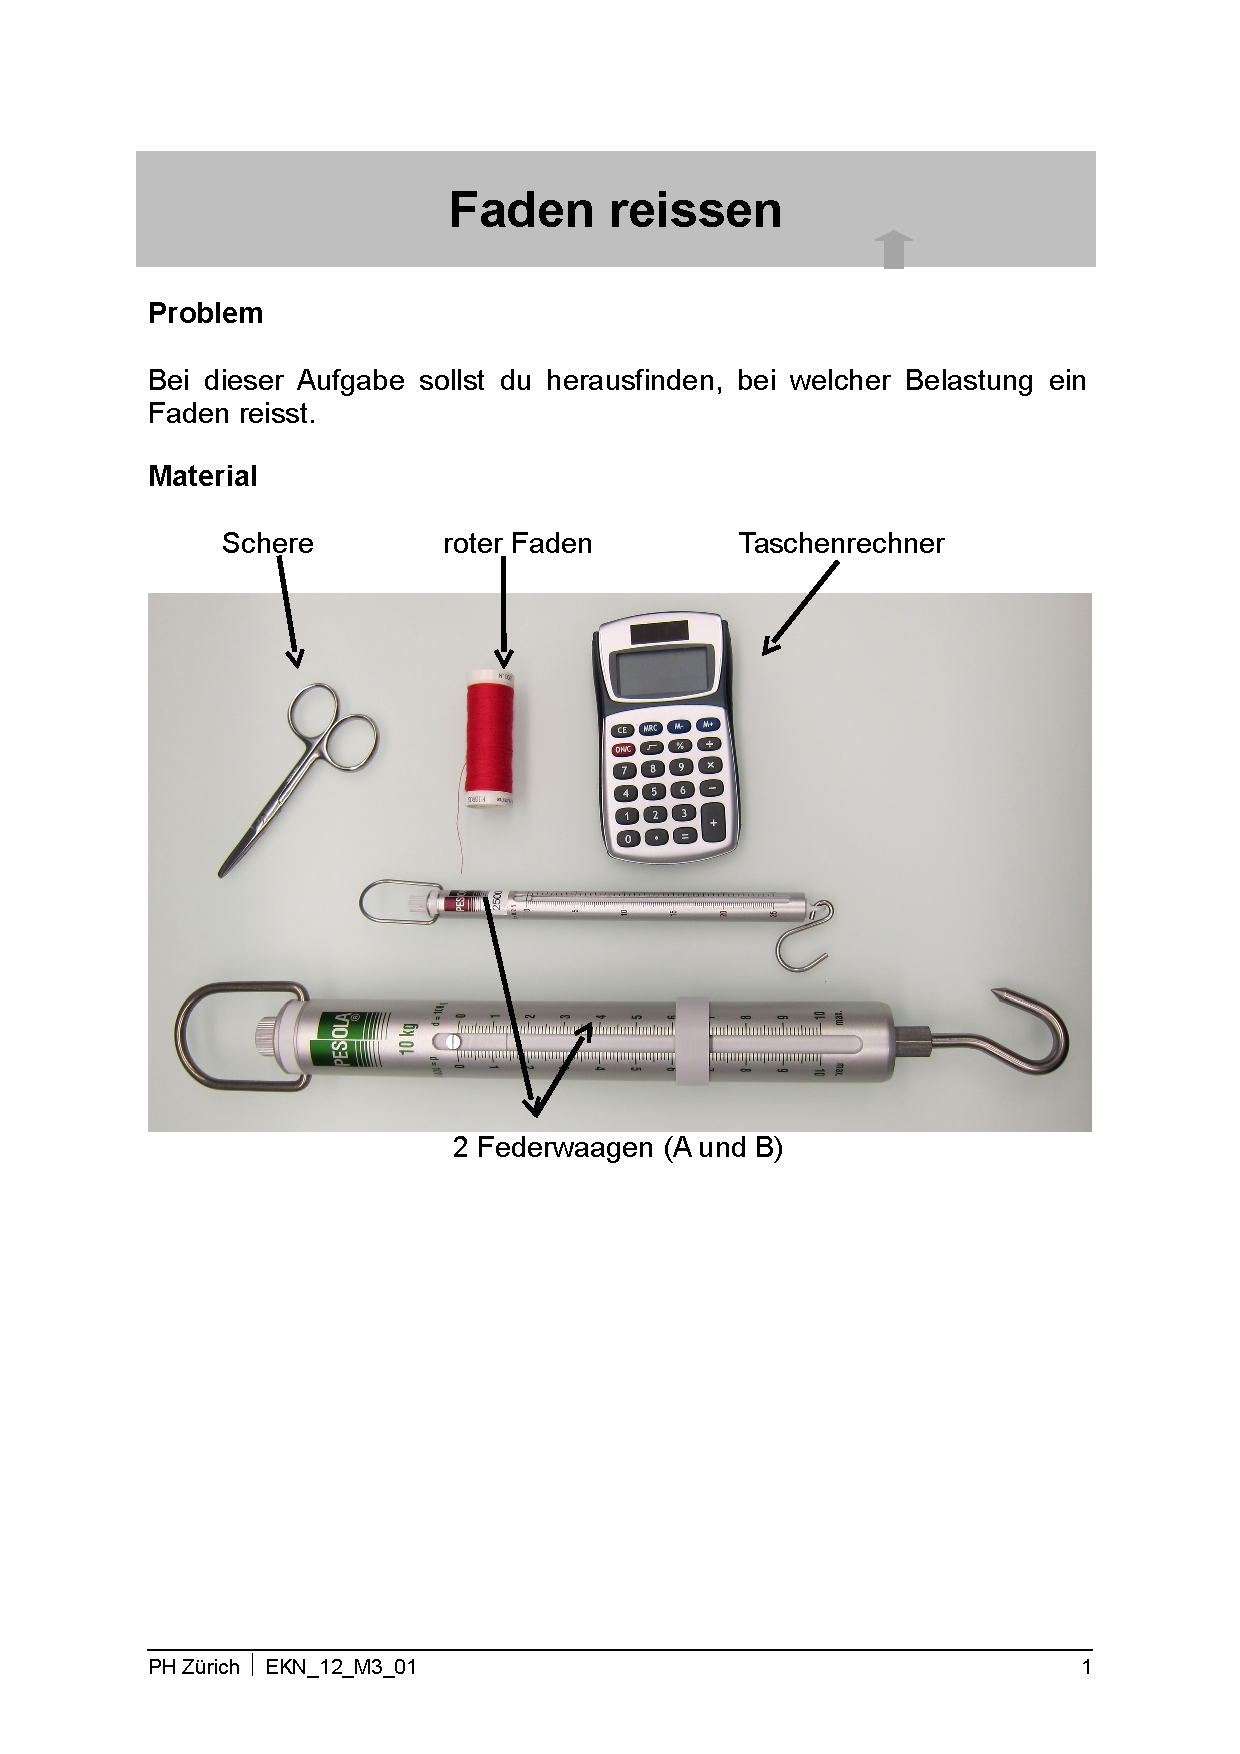
\includepdf[pages=1,pagecommand={\pagestyle{fancy}\subsection{Test 301: Aufgabenstellung}},scale=0.8]{./graphics/Test_B.pdf} 
\includepdf[pages=2-,pagecommand={\pagestyle{fancy}},scale=0.8]{./graphics/Test_B.pdf} 

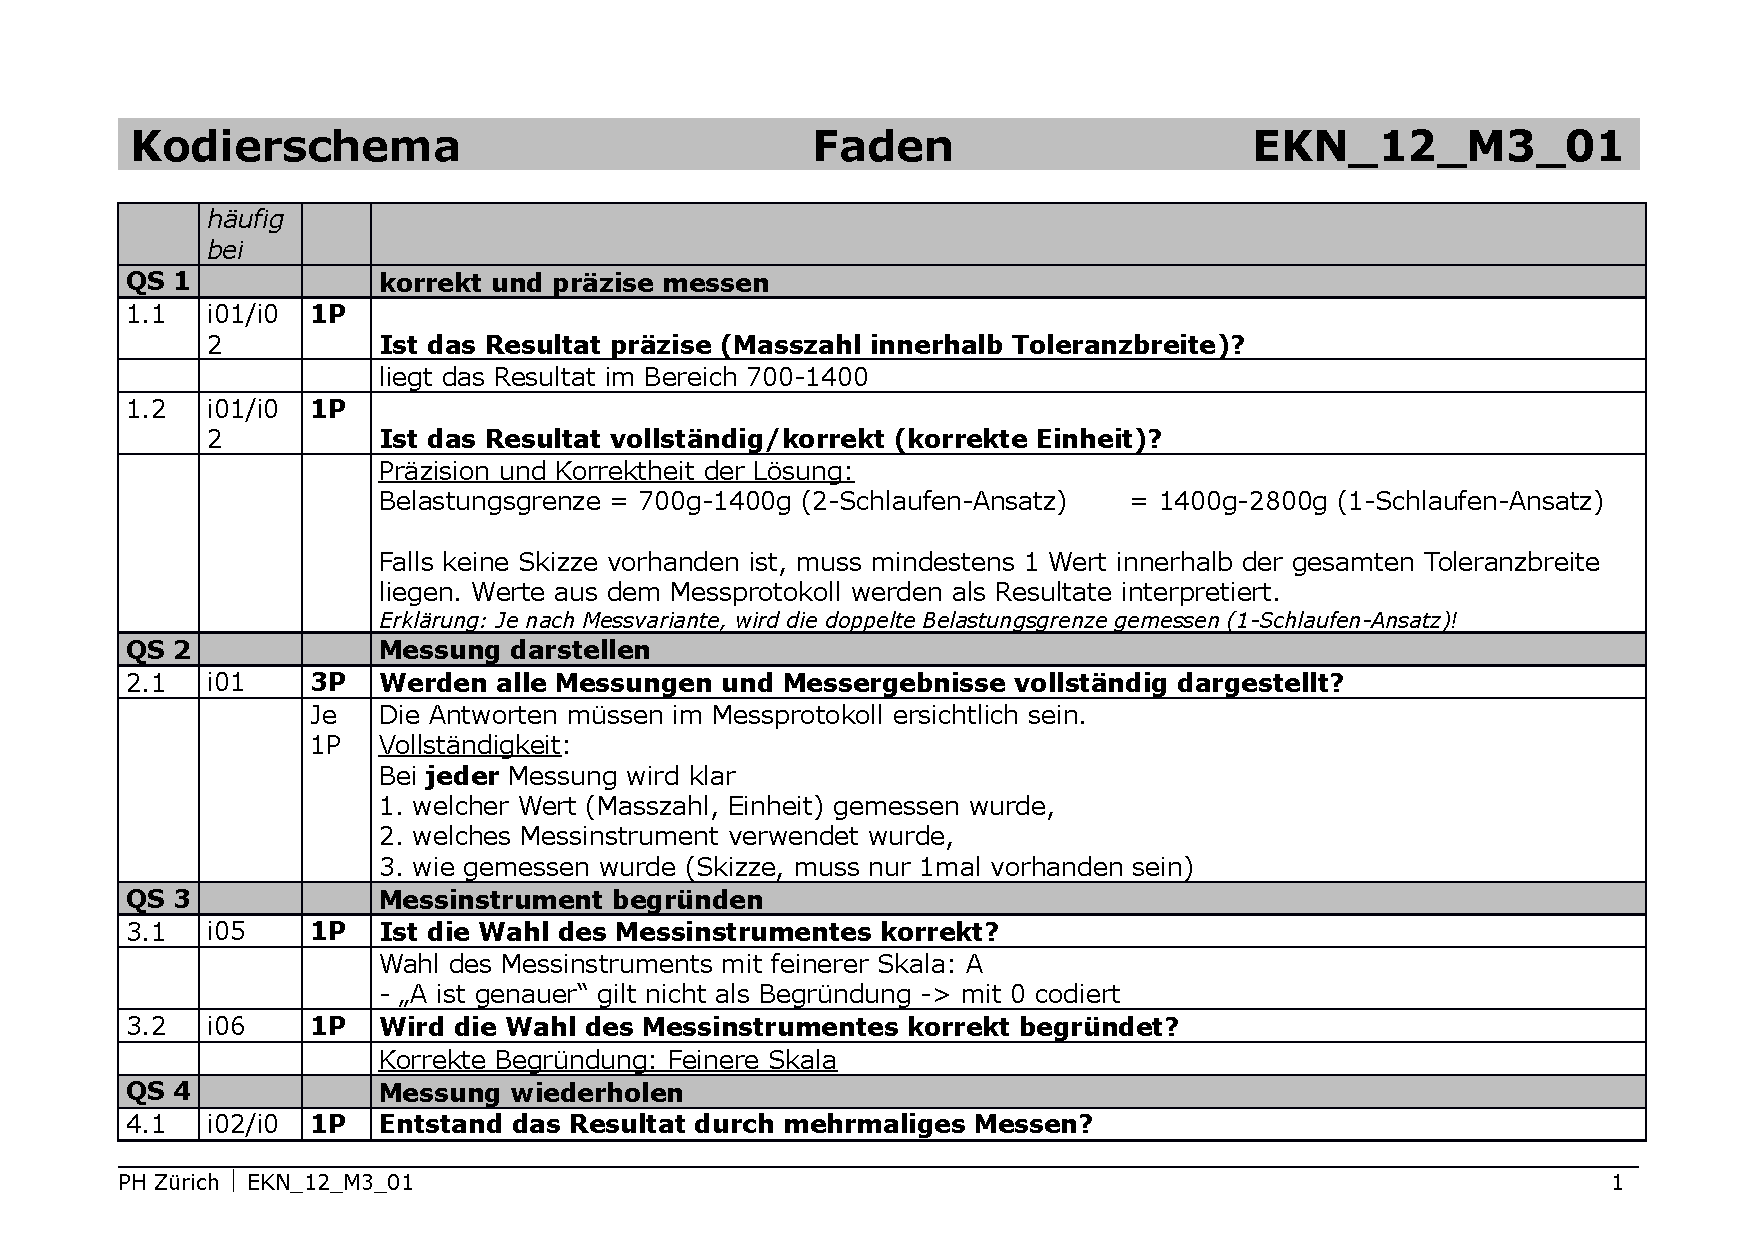
\includepdf[pages=1,pagecommand={\pagestyle{fancy}\subsection{Test 301: Kodierung}},scale=0.8]{./graphics/EKN_12_M3_Kodierschema_neu.pdf} 
\includepdf[pages=2-,pagecommand={\pagestyle{fancy}},scale=0.8]{./graphics/EKN_12_M3_Kodierschema_neu.pdf} des


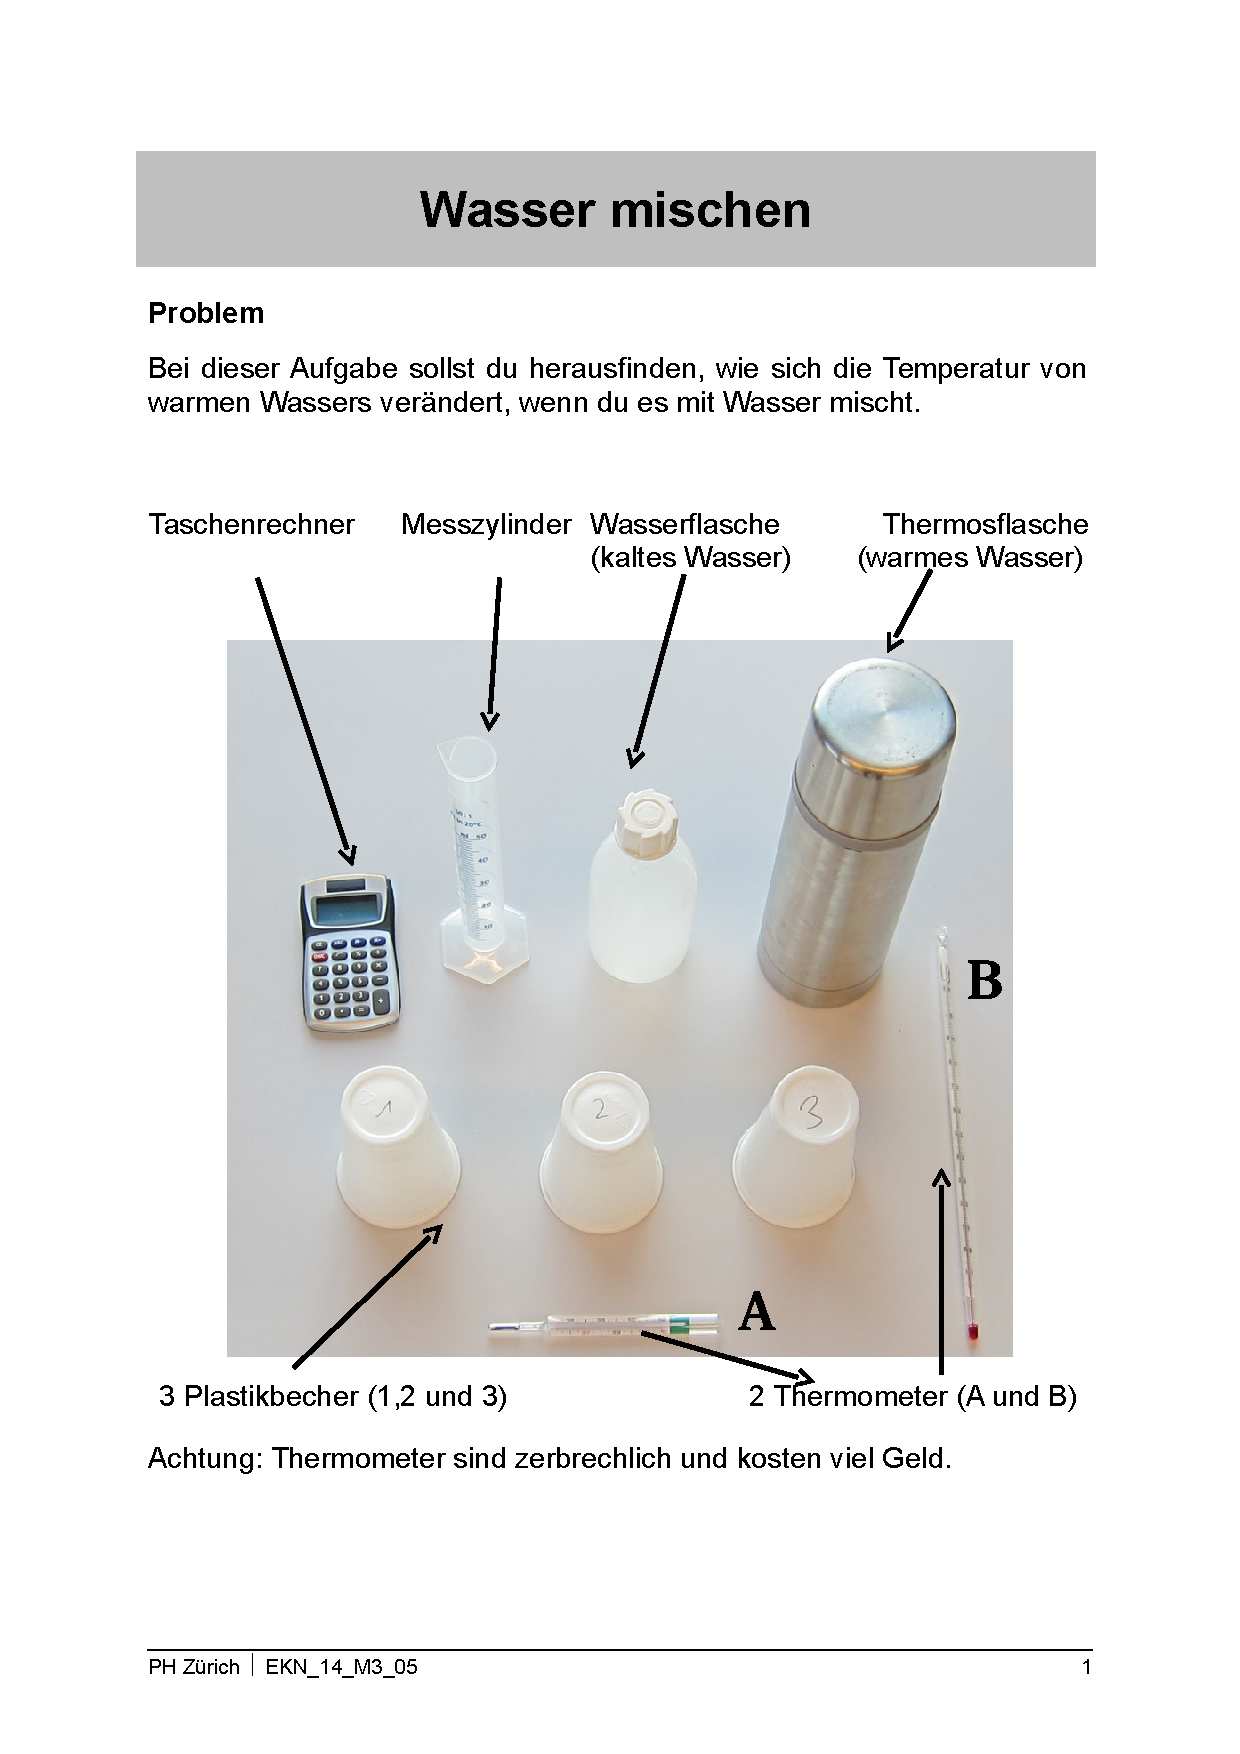
\includepdf[pages=1,pagecommand={\pagestyle{fancy}\subsection{Test 305: Aufgabenstellung}},scale=0.8]{./graphics/Test_A.pdf} 
\includepdf[pages=2-,pagecommand={\pagestyle{fancy}},scale=0.8]{./graphics/Test_A.pdf} 

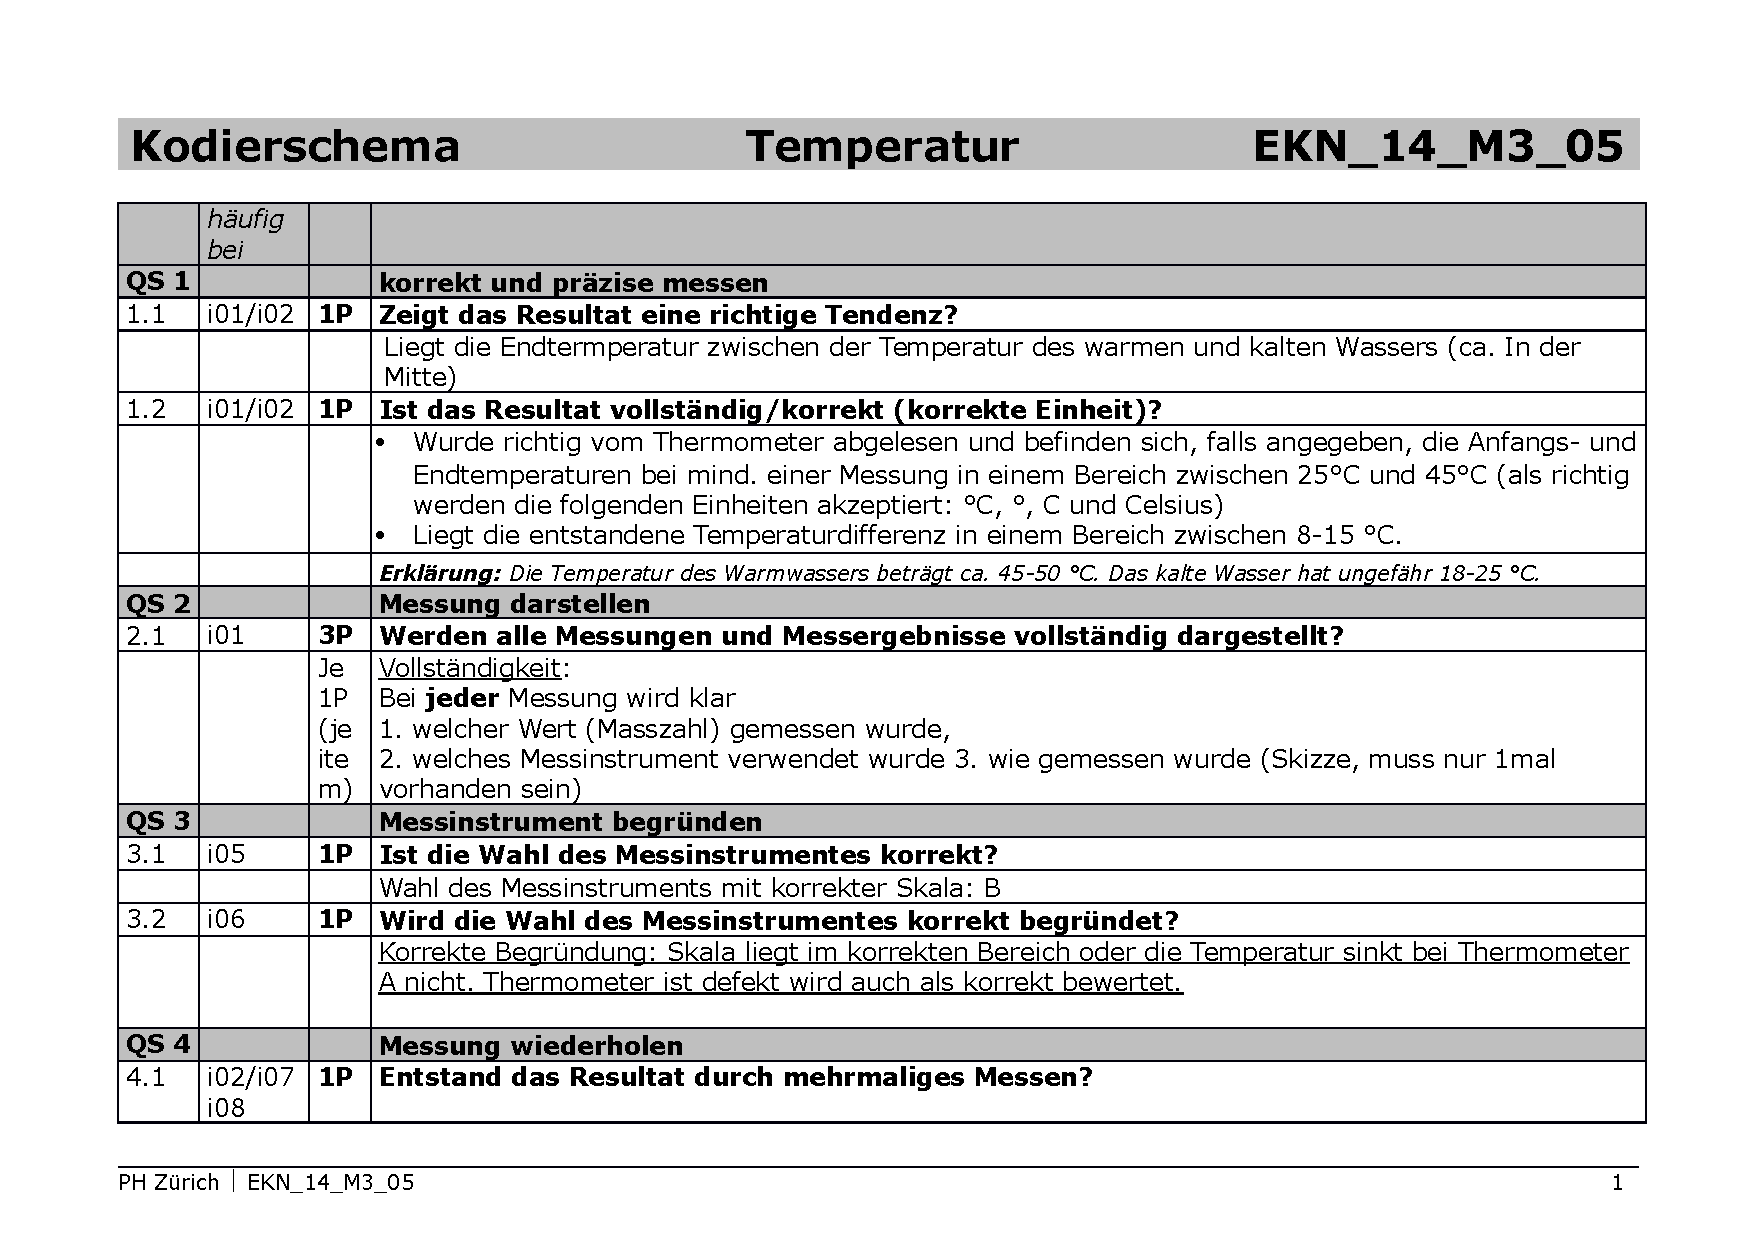
\includepdf[pages=1,pagecommand={\pagestyle{fancy}\subsection{Test 305: Kodierung}},scale=0.8]{./graphics/EKN_12_M2_Kodierschema_Physik_Temperatur.pdf} 
\includepdf[pages=2-,pagecommand={\pagestyle{fancy}},scale=0.8]{./graphics/EKN_12_M2_Kodierschema_Physik_Temperatur.pdf} 

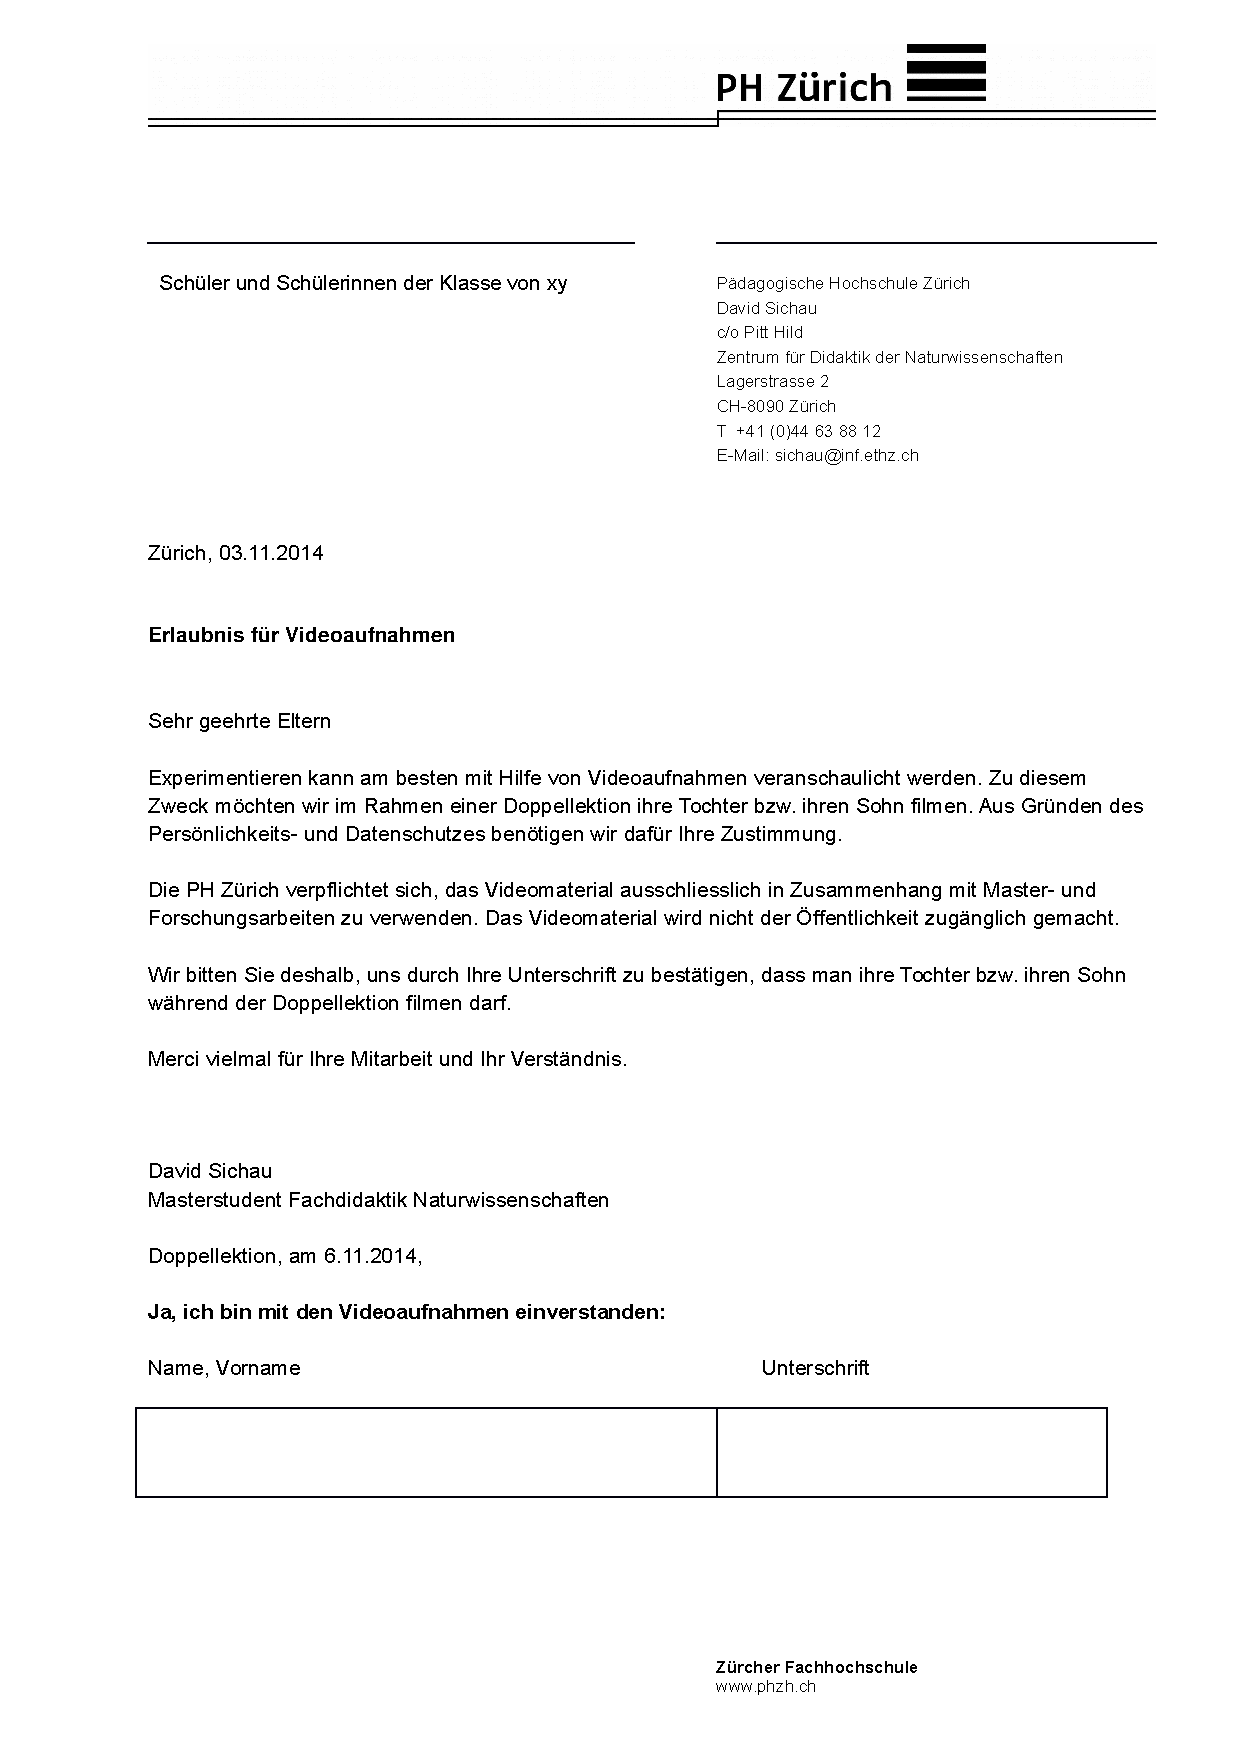
\includepdf[pages=1,pagecommand={\pagestyle{fancy}\section{Einverständnis Erklärung für Video Aufnahme}},scale=0.78]{./graphics/Erlaubnis_Videoaufnahmen.pdf} 